\documentclass[11pt]{standalone}
\usepackage{amssymb}
\usepackage{amsmath}
\usepackage[no-math]{fontspec}
\usepackage{unicode-math}
\usepackage{libertinus}
\usepackage{pgf,xcolor}
\usepackage{tikz}
\usetikzlibrary{arrows.meta, backgrounds, decorations.pathmorphing, patterns}
\usepackage{pgfplots}
\pgfplotsset{compat=newest}

\definecolor{my_darkgray}{HTML}{484949}
\definecolor{my_lightgray}{HTML}{F3F4F4}
\definecolor{my_darkblue}{HTML}{005A94}
\definecolor{my_lightblue}{HTML}{CCDEE9}
\definecolor{my_yellow}{HTML}{FFEC7F}
\definecolor{my_red}{HTML}{E60000}
\definecolor{my_orange}{HTML}{E87846}

\begin{document}

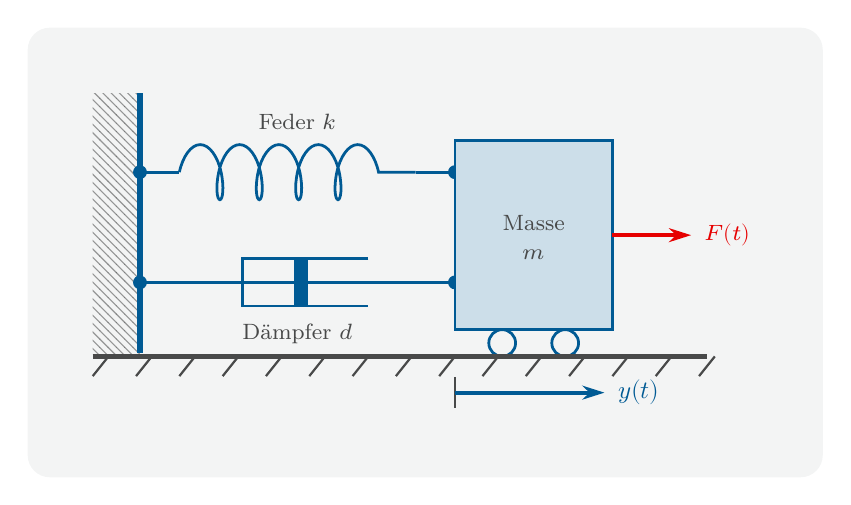
\begin{tikzpicture}[
    show background rectangle,
    background rectangle/.style={fill=my_lightgray, rounded corners=8pt},
    inner frame sep=0.8cm
]

% -------- Fixed wall ----------------------------------------
\fill[pattern=north west lines, pattern color=my_darkgray, opacity=0.55]
    (-0.6, -1.5) rectangle (0, 1.8);
\draw[my_darkblue, line width=2pt] (0, -1.5) -- (0, 1.8);

% -------- Spring (Feder, Federkonstante k) at y = 0.8 -------
% Short horizontal connectors (wall face -> coil, coil -> mass face)
\draw[my_darkblue, line width=1pt] (0, 0.8) -- (0.5, 0.8);
\draw[my_darkblue, line width=1pt,
      decorate,
      decoration={coil, amplitude=3.5mm, segment length=5mm, aspect=0.4}]
    (0.5, 0.8) -- (3.5, 0.8);
\draw[my_darkblue, line width=1pt] (3.5, 0.8) -- (4.0, 0.8);
% Attachment dots
\fill[my_darkblue] (0,   0.8) circle (2.5pt);
\fill[my_darkblue] (4.0, 0.8) circle (2.5pt);
% Label (above the coil; anchor=south keeps text clear of the coil peaks)
\node[my_darkgray, anchor=south] at (2.0, 1.22)
    {\footnotesize Feder~$k$};

% -------- Dashpot (Dämpfer, Dämpfungskonstante d) at y = -0.6
% Left connector: wall face to cylinder
\draw[my_darkblue, line width=1pt] (0, -0.6) -- (2.3, -0.6);
% Cylinder body: three sides drawn explicitly, open on the right
% so that the piston rod is seen to exit
\draw[my_darkblue, line width=1pt]
    (2.9, -0.3) -- (1.3, -0.3) -- (1.3, -0.9) -- (2.9, -0.9);
% Piston plate (thick vertical segment inside the cylinder)
\draw[my_darkblue, line width=5pt, line cap=butt]
    (2.05, -0.3) -- (2.05, -0.9);
% Piston rod: piston to right face of mass
\draw[my_darkblue, line width=1pt] (2.05, -0.6) -- (4.0, -0.6);
% Attachment dots
\fill[my_darkblue] (0,   -0.6) circle (2.5pt);
\fill[my_darkblue] (4.0, -0.6) circle (2.5pt);
% Label (below the cylinder, anchor=north keeps text below the bottom wall)
\node[my_darkgray, anchor=north] at (2.0, -1.0)
    {\footnotesize Dämpfer~$d$};

% -------- Mass block (Masse m) ------------------------------
\fill[my_lightblue]     (4, -1.2) rectangle (6, 1.2);
\draw[my_darkblue, line width=1pt] (4, -1.2) rectangle (6, 1.2);
\node[my_darkgray]              at (5,  0.15) {\footnotesize Masse};
\node[my_darkgray]              at (5, -0.25) {\footnotesize $m$};

% -------- External force F(t) -------------------------------
\draw[my_red, line width=1.5pt, -{Stealth[length=8pt, width=5pt]}]
    (6.0, 0.0) -- (7.0, 0.0);
\node[my_red, anchor=west] at (7.05, 0.0) {\footnotesize $F(t)$};

% -------- Rollers and floor ---------------------------------
% Two rolling supports under the mass (keep friction out of the model)
\draw[my_darkblue, line width=1pt, fill=my_lightgray]
    (4.6, -1.37) circle (0.17);
\draw[my_darkblue, line width=1pt, fill=my_lightgray]
    (5.4, -1.37) circle (0.17);
% Floor line
\draw[my_darkgray, line width=1.5pt] (-0.6, -1.54) -- (7.2, -1.54);
% Ground hatching (14 short diagonal lines, spacing 0.55 cm)
\foreach \i in {0,...,14} {
    \draw[my_darkgray, line width=0.8pt]
        ({-0.4 + \i * 0.55}, -1.54) -- ({-0.6 + \i * 0.55}, -1.79);
}

% -------- Displacement coordinate y(t) ----------------------
% Reference tick at the equilibrium position (left face of mass)
\draw[my_darkgray, line width=1pt] (4, -1.80) -- (4, -2.2);
% Arrow in the positive-y direction (hier: Bewegungsrichtung nach rechts)
\draw[my_darkblue, line width=1.5pt, -{Stealth[length=8pt, width=5pt]}]
    (4, -2.0) -- (5.9, -2.0);
\node[my_darkblue, anchor=west] at (5.95, -2.0) {\small $y(t)$};

\end{tikzpicture}

\end{document}